\chapter{Asking Bugatti Owners How They Got RICH!}

These notes follow Lecture 49 of the School of Hard Knocks interview series, curated here by LazyingArt LLC. The lecture proceeds with more discipline than its street-interview surface first suggests. It begins by spending astonishment, then converts astonishment into a search for method. A Bugatti, a few violent numerical claims, and a wealthy city are made to serve as the opening data. Only after that does the lecture begin asking what mechanism, what business structure, and what kind of human temperament could plausibly sit behind the numbers.

\section{Bugatti, Scottsdale, and the Promise of a Method}

The cold open is a montage. We should therefore resist the temptation to read its quantities as if they came from one speaker and one argument. Their function is preparatory. The lecture wants to create a field of tension before it explains anything. A luxury object appears, and then, in rapid succession, we are given a case value, a one-day business number, and a later after-tax income claim:

\begin{align}
V_{\text{Deepwater}}&=\$28\,\text{million},\\
R_{\text{day}}&=\$80\,\text{million},\\
Y_{\text{after-tax}}&=\$15\,\text{million},\\
T_{\text{federal}}&=0.
\end{align}

Each quantity belongs to a different local claim. One refers to the Deepwater Horizon case. One refers to a day in the car business. One refers to a personal after-tax year. One refers to federal income tax as later described by a real-estate investor. The lecture deliberately stacks them before it tells us how to sort them.

\begin{figure}
\centering
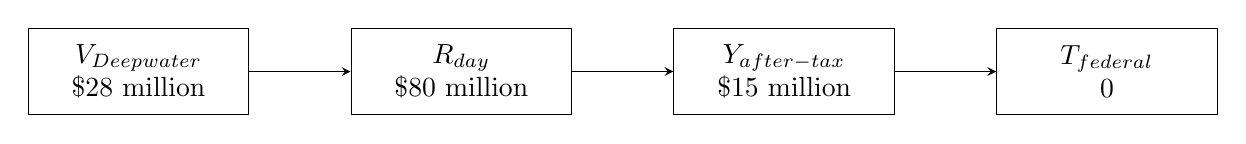
\begin{tikzpicture}[>=stealth]
\node[draw, rectangle, align=center, minimum width=2.8cm, minimum height=1.1cm] (a) at (0,0) {$V_{\text{Deepwater}}$\\$\$28$ million};
\node[draw, rectangle, align=center, minimum width=2.8cm, minimum height=1.1cm] (b) at (4.1,0) {$R_{\text{day}}$\\$\$80$ million};
\node[draw, rectangle, align=center, minimum width=2.8cm, minimum height=1.1cm] (c) at (8.2,0) {$Y_{\text{after-tax}}$\\$\$15$ million};
\node[draw, rectangle, align=center, minimum width=2.8cm, minimum height=1.1cm] (d) at (12.3,0) {$T_{\text{federal}}$\\$0$};
\draw[->] (a) -- (b);
\draw[->] (b) -- (c);
\draw[->] (c) -- (d);
\end{tikzpicture}
\end{figure}

Only after this numerical strip does the host reset the stage. We are in Scottsdale, Arizona, and the promise is stated cleanly: the lecture will move from spectacle to blueprint. Wealthy operators will be asked how they built their money, and the viewer will be invited to extract a usable method. The rest of the chapter should be read with that promise in mind. Each interview is a mini-case. First a business line is named. Then a number lands. Then the host sharpens toward mechanism.

\section{The First Operator: Capital, Land, and Concentration}

The first full interview begins with a joke about never having been broke and then almost immediately turns serious. The speaker is in many businesses, but commercial real estate is the line he names first. The host presses on a familiar obstacle: people say one needs a lot of capital to begin.

\subsection{Question \& Answer}

\paragraph{Question.} Do we really need a great deal of capital to get started?

\paragraph{Answer.} The lecture's answer here is not a universal theorem that money never matters. It is narrower and more pointed. The speaker rejects capital as the primary explanatory variable and replaces it with judgment, hard work, and the willingness to attack when conditions fall apart. In other words, he moves the argument from passive endowment to operating capacity.

The host tests that rhetoric immediately with a quantity. The number given is explicitly personal rather than corporate:

\begin{equation}
Y_{\text{self,max}}=\$3.75\,\text{million}.
\end{equation}

That distinction should remain visible. The lecture is not yet asking for company turnover. It is asking what one person actually made.

The speaker then explains why real estate became his vehicle. It was not a theory chosen in the abstract. He had expected to move toward stocks, interviewed at Grub \& Ellis, and entered commercial real estate because land was the available opening. The local fit mattered. A ranching and farming background in western Kansas meant that he already understood the people who moved in that market. This is one of the lecture's recurring lessons: an industry can become legible to us because some earlier life has already trained our eye.

The interview now narrows again, from industry choice to relationship structure.

\subsection{Question \& Answer}

\paragraph{Question.} Why can a very small client base be enough in a high-ticket business?

\paragraph{Answer.} Because the relevant quantity is not the sheer count of contacts but the concentration of meaningful transactions in a small repeating set. The speaker says that in his business one may only need two or three serious clients. We may represent that schematically as

\begin{equation}
N_{\text{core clients}}\approx 2\text{ to }3,
\qquad
R_{\text{total}}=\sum_{i=1}^{N_{\text{core clients}}}R_i,
\qquad
N_{\text{core clients}}\ll 1000.
\end{equation}

The summation is only a clean reconstruction of the idea. The lecture does not provide a ledger. What it does provide is a business logic: a few large, trusted, repeat relationships can dominate total income.

\begin{figure}
\centering
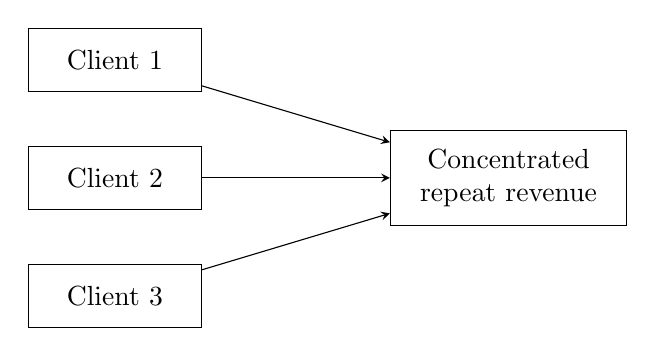
\begin{tikzpicture}[>=stealth]
\node[draw, rectangle, minimum width=2.2cm, minimum height=0.8cm] (c1) at (0,1.5) {Client 1};
\node[draw, rectangle, minimum width=2.2cm, minimum height=0.8cm] (c2) at (0,0) {Client 2};
\node[draw, rectangle, minimum width=2.2cm, minimum height=0.8cm] (c3) at (0,-1.5) {Client 3};
\node[draw, rectangle, align=center, minimum width=3.0cm, minimum height=1.2cm] (rev) at (5,0) {Concentrated\\repeat revenue};
\draw[->] (c1) -- (rev);
\draw[->] (c2) -- (rev);
\draw[->] (c3) -- (rev);
\end{tikzpicture}
\end{figure}

The remainder of the interview compresses this business logic into character. The speaker dismisses the authority of professors, insists that ``never quit'' is a real separator, and explains confidence not as fantasy but as something that followed results. Faith arrives late in the sequence, just as it does in the interview. It was not the first instrument, but it becomes, by the speaker's own account, indispensable.

\section{The Car Business: Iteration, Truth, and Reputation}

A sponsor interruption breaks the lecture's motion. That interruption matters structurally because the lecture restarts itself correctly: not with abstraction, but with another Bugatti and another number. The new speaker is in the car business, and the host again asks for the largest amount of money made in a single year. The answer remains arresting:

\begin{equation}
R_{\text{day}}=\$80\,\text{million}.
\end{equation}

We are not told whether this is gross sales, total volume, or some other measure of a day's business. The correct procedure is therefore to keep the number narrow and speaker-attributed. The lecture itself does not over-define it.

From here the interview makes a very interesting turn. The host asks about school, and the speaker says he was a bad student and had ADD before the term was commonly recognized. The business interpretation he places on this is not deficiency but asymmetry: creativity, vision, and energy at the center, stabilized by calmer and more focused people around him. The lecture does not give us a typology worth formalizing, but it does give us a clear bias toward experiment over perfection.

\subsection{Question \& Answer}

\paragraph{Question.} What is the business value of experimentation over perfection?

\paragraph{Answer.} The lecture answers with a contrast. One model launches, fails, learns, and launches again. Another waits years for a single perfect attempt and may still fail. As a compact reconstruction of that doctrine we may write

\begin{equation}
\text{iteration}\to\text{failure}\to\text{learning}\to\text{improvement}.
\end{equation}

This is not a theorem. It is a business state diagram. The point is not rockets as such. The point is that the market teaches those who are willing to expose an incomplete attempt to reality.

\begin{figure}
\centering
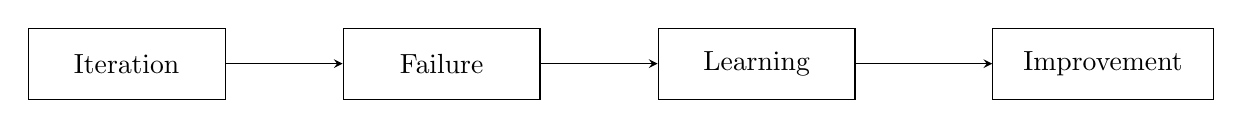
\begin{tikzpicture}[>=stealth]
\node[draw, rectangle, minimum width=2.5cm, minimum height=0.9cm] (a) at (0,0) {Iteration};
\node[draw, rectangle, minimum width=2.5cm, minimum height=0.9cm] (b) at (4,0) {Failure};
\node[draw, rectangle, minimum width=2.5cm, minimum height=0.9cm] (c) at (8,0) {Learning};
\node[draw, rectangle, minimum width=2.8cm, minimum height=0.9cm] (d) at (12.4,0) {Improvement};
\draw[->] (a) -- (b);
\draw[->] (b) -- (c);
\draw[->] (c) -- (d);
\end{tikzpicture}
\end{figure}

But iteration alone is not enough. The second half of the interview turns from experimentation to trust.

\subsection{Question \& Answer}

\paragraph{Question.} What creates trust in a high-ticket sales business?

\paragraph{Answer.} The answer is unusually plain: tell the truth, under-promise, over-deliver, and keep your word. The lecture then supplies an empirical sign that this doctrine is working. A buyer in Dubai reports that the cars arrive better than described, not worse, and therefore he is comfortable buying sight unseen. Trust, then, lowers verification cost and widens the field of possible transactions.

This is the right way to read the handshake doctrine that follows. It is not merely nostalgia for a more honorable age. It is a market argument. Honest description and reliable performance create repeat business and permit transactions that would otherwise be too friction-heavy to occur.

The speaker then broadens the doctrine into life design. The choice of spouse is described as a structural variable in the enterprise. If the nearest relationship fights the work, friction rises. If it joins the work, the whole system becomes easier to sustain. The interview closes on a generational note, but even there the underlying concern is the same one we have seen already: whether an ethic of work, trust, and risk still survives.

\section{Out-of-the-Box Improvement and the Search for a Better Way}

The next interview changes the atmosphere without changing the lecture's deeper structure. We are still being asked what generates wealth, but now the answer is neither asset-class prestige nor pure salesmanship. The speaker presents himself as a man who refuses the box. He says, with a kind of deliberate eccentricity, that he thinks out of the box and even ``builds triangles.'' We should not literalize the geometry. The point is that value appears when the given arrangement of work is treated as alterable.

The origin story is severe. In 1970 he is sleeping in his car and saying there must be a better way. At McDonald's he sees twelve people in a workflow, changes the spatulas, changes where the buns are placed, and changes the flow of movement. The lecture does not try to beautify this. It wants us to feel the directness of the impulse: if a process wastes motion, alter the process.

The speaker later ties that same instinct to a much larger outcome:

\begin{equation}
V_{\text{Deepwater}}=\$28\,\text{million}.
\end{equation}

We are not given the fee structure or the detailed legal mechanics of the case. The lecture's point is narrower. Small redesigns and a constant attention to improvement can scale upward into very large commercial results.

\subsection{Question \& Answer}

\paragraph{Question.} How does constant process improvement become a wealth engine?

\paragraph{Answer.} By turning every awkward process into a candidate for redesign. The lecture does not offer a formal productivity function. It offers a more primitive and in some ways more useful operating habit: every time a process feels clumsy, ask what geometry of action would make it less clumsy.

That same style governs the negotiation doctrine in the interview. The usable business content is compressed into one line: ``100\% honesty, period.'' The surrounding rhetoric should not be elevated into doctrine. The stable element is honesty. Speech must line up with reality. Otherwise negotiation becomes theatrical and wealth-producing trust disappears.

The host then asks how the speaker escaped poverty. The answer returns, with almost no ornament, to the first question: ask for a better way, stay sober, stay moving, and keep asking what one can provide that other people have not yet imagined.

\section{Pace Morby: Tax Law, Seller Finance, and Cash Flow}

With Pace Morby the lecture reaches its most explicit mathematical core. The host introduces him as a major real-estate entrepreneur and asks operational questions in the right order: why real estate, how much money he has made, how it is possible to pay zero federal income tax, why the arrangement is legal, and how one can buy property without a bank, without credit, and without cash out of pocket.

The numerical frame is wide enough that we should collect it first:

\begin{align}
t_{\text{real estate}}&=12\ \text{years},
&
t_{\text{construction prior}}&=10\ \text{years},\\
Y_{\text{after-tax}}&=\$15\,\text{million},
&
R_{\text{company}}&\approx \$115\,\text{million}\ \text{per year},\\
P_{\text{portfolio}}&\approx \$500\,\text{million}.&
\end{align}

The central tax claim is then stated:

\begin{align}
Y_{\text{after-tax}}&=Y_{\text{pre-tax}}-T_{\text{federal}}-T_{\text{other}},\\
T_{\text{federal}}&=0,
\qquad
\Delta t_{\text{no federal tax}}=7\ \text{years}.
\end{align}

\begin{remark}
The lecture is precise at exactly one point here. Federal income tax is claimed to be zero. Other taxes are not. Pace explicitly says that property taxes and employment taxes remain. The argument is therefore about the tax treatment of real-estate investment, not about the disappearance of all taxation.
\end{remark}

The lecture next connects that tax claim to a public-policy comparison:

\begin{equation}
C_{\text{gov,unit}}\approx \$600{,}000,
\qquad
C_{\text{private,unit}}\approx \$75{,}000,
\qquad
\frac{C_{\text{gov,unit}}}{C_{\text{private,unit}}}\approx 8.
\end{equation}

This is a strong rhetorical comparison, but not a complete cost model. We should preserve the ratio as a speaker-attributed claim and nothing more.

Now the lecture turns from tax law to acquisition mechanism.

\subsection{Question \& Answer}

\paragraph{Question.} How can real estate produce large after-tax cash flow with no bank, no credit, and no cash out of pocket?

\paragraph{Answer.} The lecture's answer is seller finance. The logic is sequential and, at least at the level stated in the interview, quite clean.

\begin{enumerate}
\item A long-time owner wants to retire and prefers a monthly check.
\item A cash sale would produce a large immediate capital-gains event.
\item Seller finance lets that owner act as lender rather than as a party exiting all at once.
\item Rent from tenants services the obligation and leaves a residual cash flow if the property is operated correctly.
\end{enumerate}

For compactness we may write the buyer's stated entry conditions as

\begin{equation}
L_{\text{bank}}=0,
\qquad
X_{\text{credit}}=0,
\qquad
K_{\text{out}}=0.
\end{equation}

That is editorial shorthand, not the speaker's own notation. It is simply a clean way of preserving the doctrine.

\begin{figure}
\centering
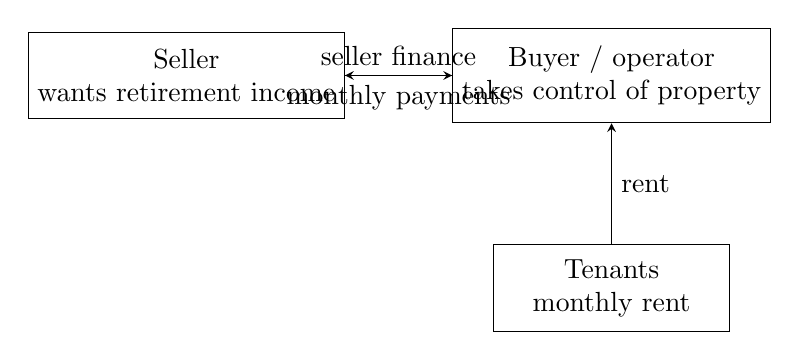
\begin{tikzpicture}[>=stealth]
\node[draw, rectangle, align=center, minimum width=3.0cm, minimum height=1.1cm] (seller) at (0,0) {Seller\\wants retirement income};
\node[draw, rectangle, align=center, minimum width=3.8cm, minimum height=1.2cm] (buyer) at (5.4,0) {Buyer / operator\\takes control of property};
\node[draw, rectangle, align=center, minimum width=3.0cm, minimum height=1.1cm] (tenants) at (5.4,-2.7) {Tenants\\monthly rent};
\draw[->] (seller) -- node[above]{seller finance} (buyer);
\draw[->] (buyer) -- node[below]{monthly payments} (seller);
\draw[->] (tenants) -- node[right]{rent} (buyer);
\end{tikzpicture}
\end{figure}

\paragraph{Worked example.} The lecture then gives the clearest numerical example in the entire chapter. One property has

\begin{equation}
N_{\text{units}}=160,
\qquad
R_{\text{gross,month}}\approx \$160{,}000,
\qquad
CF_{\text{net,month}}\approx \$53{,}000.
\end{equation}

The cash-flow identity we need is

\begin{equation}
CF_{\text{net}}
=
R_{\text{tenants}}
-
P_{\text{seller}}
-
C_{\text{tax}}
-
C_{\text{insurance}}
-
C_{\text{management}}
-
C_{\text{repairs}}.
\end{equation}

If we treat the stated gross monthly figure as tenant revenue, then the combined outflow is reconstructed by subtraction:

\begin{align}
P_{\text{seller}}+C_{\text{tax}}+C_{\text{insurance}}+C_{\text{management}}+C_{\text{repairs}}
&\approx R_{\text{gross,month}}-CF_{\text{net,month}}\\
&\approx \$160{,}000-\$53{,}000\\
&\approx \$107{,}000.
\end{align}

This is all the lecture strictly licenses us to compute, but it is enough to produce one informative scale ratio:

\begin{equation}
\frac{CF_{\text{net,month}}}{R_{\text{gross,month}}}
\approx
\frac{53}{160}
\approx
0.331.
\end{equation}

Again, this is not a general theorem about real-estate margins. It is only a ratio extracted from the particular example the speaker supplies.

\begin{figure}
\centering
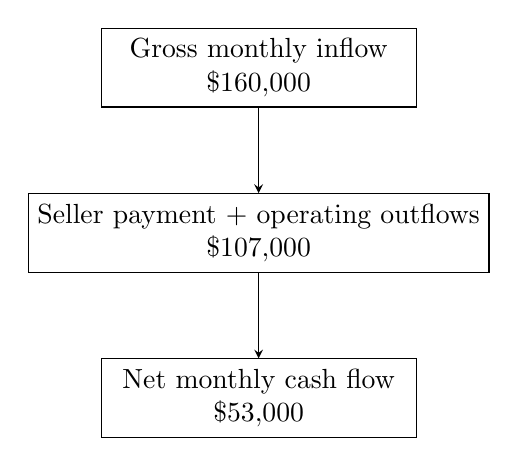
\begin{tikzpicture}[>=stealth]
\node[draw, rectangle, align=center, minimum width=4.0cm, minimum height=1.0cm] (gross) at (0,2.8) {Gross monthly inflow\\$\$160{,}000$};
\node[draw, rectangle, align=center, minimum width=4.0cm, minimum height=1.0cm] (out) at (0,0.7) {Seller payment + operating outflows\\$\$107{,}000$};
\node[draw, rectangle, align=center, minimum width=4.0cm, minimum height=1.0cm] (net) at (0,-1.4) {Net monthly cash flow\\$\$53{,}000$};
\draw[->] (gross) -- (out);
\draw[->] (out) -- (net);
\end{tikzpicture}
\end{figure}

\section{Scale, Complementarity, Permission, and Survival}

After the most technical section, the lecture does not stop. It turns back to the human arrangements that make large numbers durable. First comes delegation. Then comes hiring. Then comes complementarity in partnership. Pace's rule is memorable because it is so operational: if we pay badly, we attract weak execution; if we want scale, we must pay for quality and pair with people whose skills oppose and complete our own.

A compact reconstruction of that doctrine is

\begin{equation}
Q_{\text{scale}}
\approx
f(\text{delegation},\ \text{high-quality hires},\ \text{complementary partners}).
\end{equation}

This should be read as a heuristic, not a model. The lecture's prose is richer than the formula. One partner attracts, teaches, performs publicly, and brings people in. The other manages payroll, books, operations, and the daily integrity of the system. The enterprise grows because functions are separated well.

The lecture then moves from complementarity to permission. Pace quotes the line about a man convinced against his will remaining of the same opinion still, and the host lets that proverb do real work. The point is not merely that skeptics are annoying. The point is that trying to drag disbelief into belief can waste years that should have been spent with those already capable of seeing.

\subsection{Question \& Answer}

\paragraph{Question.} What kind of relationships make large-scale ambition durable?

\paragraph{Answer.} The lecture gives three answers. First, opposite-skill partners who complete a deficiency instead of mirroring a strength. Second, collaborators who already believe in the vision instead of those who must be convinced against their will. Third, a community that grants permission to become larger than the environment that formed us.

The chapter must not smooth away the descent that follows. Pace describes the suicide of his brother, his divorce, a family imprisonment, his own suicide note, and the phone call from his mother that interrupted the act. Only after that descent does the lecture return to arithmetic:

\begin{equation}
N_{\text{employees}}\approx 600,
\qquad
R_{\text{annual}}\approx \$100\,\text{million}.
\end{equation}

The sequence matters. The lecture does not offer arithmetic as consolation. It offers something harsher and more convincing. The same life can contain catastrophic collapse and later institutional scale. Community, on this reading, is not decoration. It is part of the machinery by which ambition survives long enough to become productive.

\section{Summary}

The lecture begins by spending surprise and ends by spending mechanism. First we are given spectacle: a Bugatti, \$28 million, \$80 million in one day, \$15 million after tax, and zero federal income tax. Then we are given doctrines: capital is not the whole story, two or three clients may dominate a business, truth compounds in sales, and improvement begins by refusing the given box. Finally we are given a more explicit construction: tax treatment, seller finance, monthly cash flow, delegation, opposite-skill partnership, and community as permission. What emerges is not a universal law of wealth. It is a chain of cases in which money, method, and character are made to explain one another step by step.